% ==============================================================================
% 05_synthese_discussion.tex - Module 5 (16h30 - 17h30)
% Question / discussion & Atelier d'ingénierie projet
% Cas concrets : BlueROV2 échantillonneur, BlueBoat bathymétrique, budget labo, règles d'or
% ==============================================================================

\section{Module 5 : Synthèse \& Discussions}

\begin{frame}{5.1 Cas Pratique 1 : Le BlueROV2 Échantillonneur Benthique}
  \begin{columns}[c]
    \begin{column}{0.35\textwidth}
      \begin{center}
        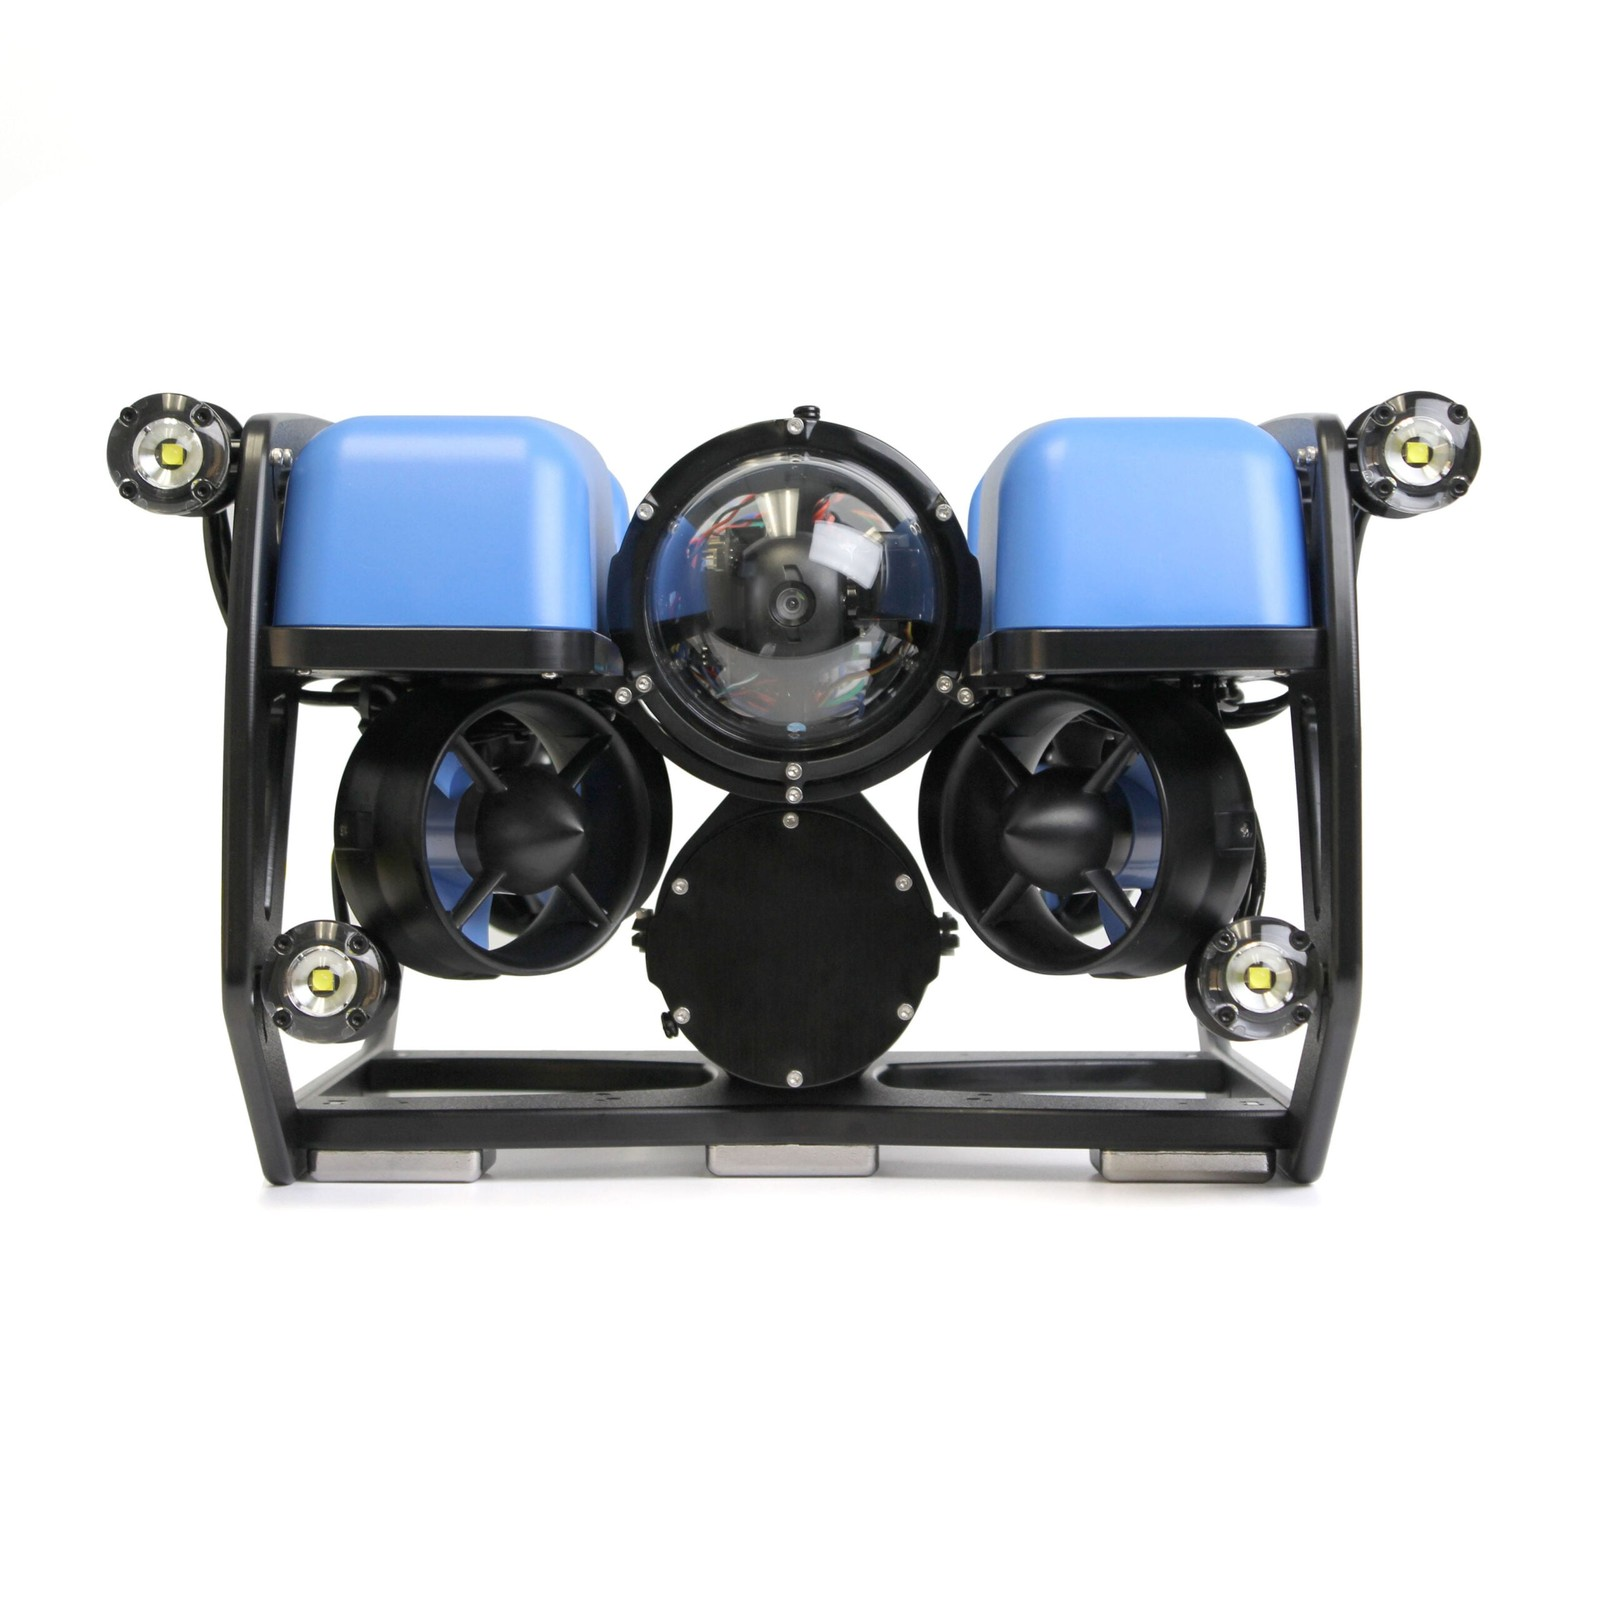
\includegraphics[height=2.0cm, keepaspectratio]{bluerov2.jpg}\\
        \vspace{0.15em}
        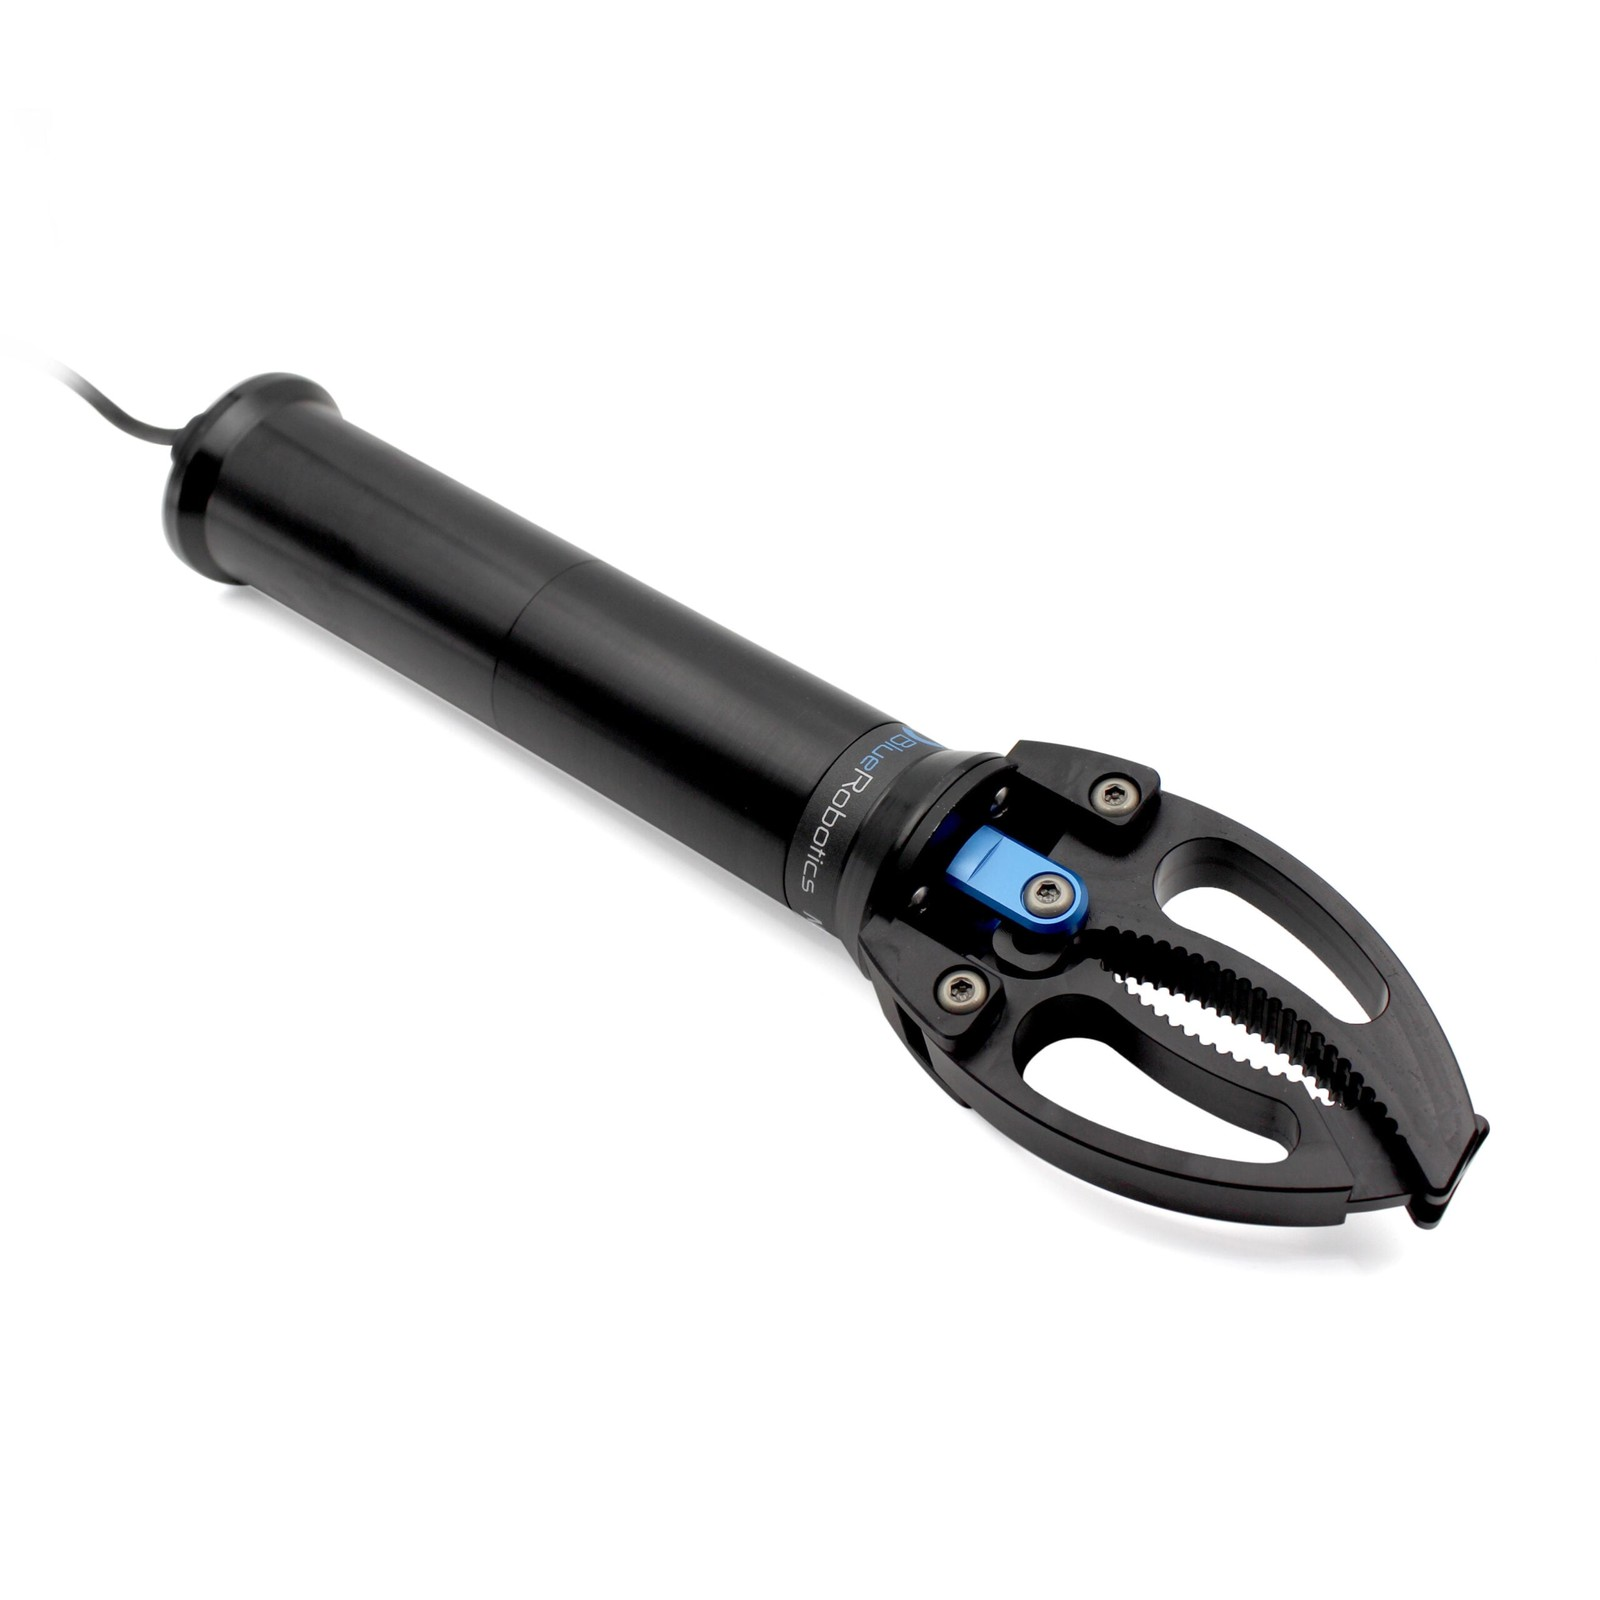
\includegraphics[height=1.7cm, keepaspectratio]{newton_gripper.jpg}\\
        \vspace{0.1em}
        \scriptsize\textbf{BlueROV2 Heavy} + \textbf{Pince Newton}
      \end{center}
    \end{column}

    \begin{column}{0.62\textwidth}
      \textbf{Architecture pour le laboratoire} :
      \scriptsize
      \begin{itemize}
        \item \textbf{Châssis 8 propulseurs (Heavy)} : contrôle complet à 6 DDL, assiette inclinée maintenue vers le fond.
        \item \textbf{Pince Newton Gripper} : préhension d'échantillons géologiques, macroalgues ou pose d'instruments.
        \item \succw{Astuce Caisson Auxiliaire 3"} : caisson 4" réservé à la navigation (jamais ouvert en mer), charge utile scientifique logée dans un caisson 3" dédié.
        \item 4 projecteurs Lumens ($6000\,\text{lm}$) pour vidéo benthique HD.
      \end{itemize}

      \vspace{0.3em}
      \begin{block}{Budget Estimatif Recherche}
        \scriptsize
        BlueROV2 Heavy ($\approx 5\text{--}7\,\text{k€}$) + Pince Newton ($\approx 700\,\text{€}$) + DVL-A50 optionnel ($\approx 6\text{--}8\,\text{k€}$).\\
        \textbf{Total} : $\approx 6\text{--}15\,\text{k€}$ contre $>40\,\text{k€}$ pour un ROV industriel fermé !
      \end{block}
    \end{column}
  \end{columns}
\end{frame}

\begin{frame}{5.2 Cas Pratique 2 : Le BlueBoat Hydrographe \& Qualité d'Eau}
  \begin{columns}[c]
    \begin{column}{0.35\textwidth}
      \begin{center}
        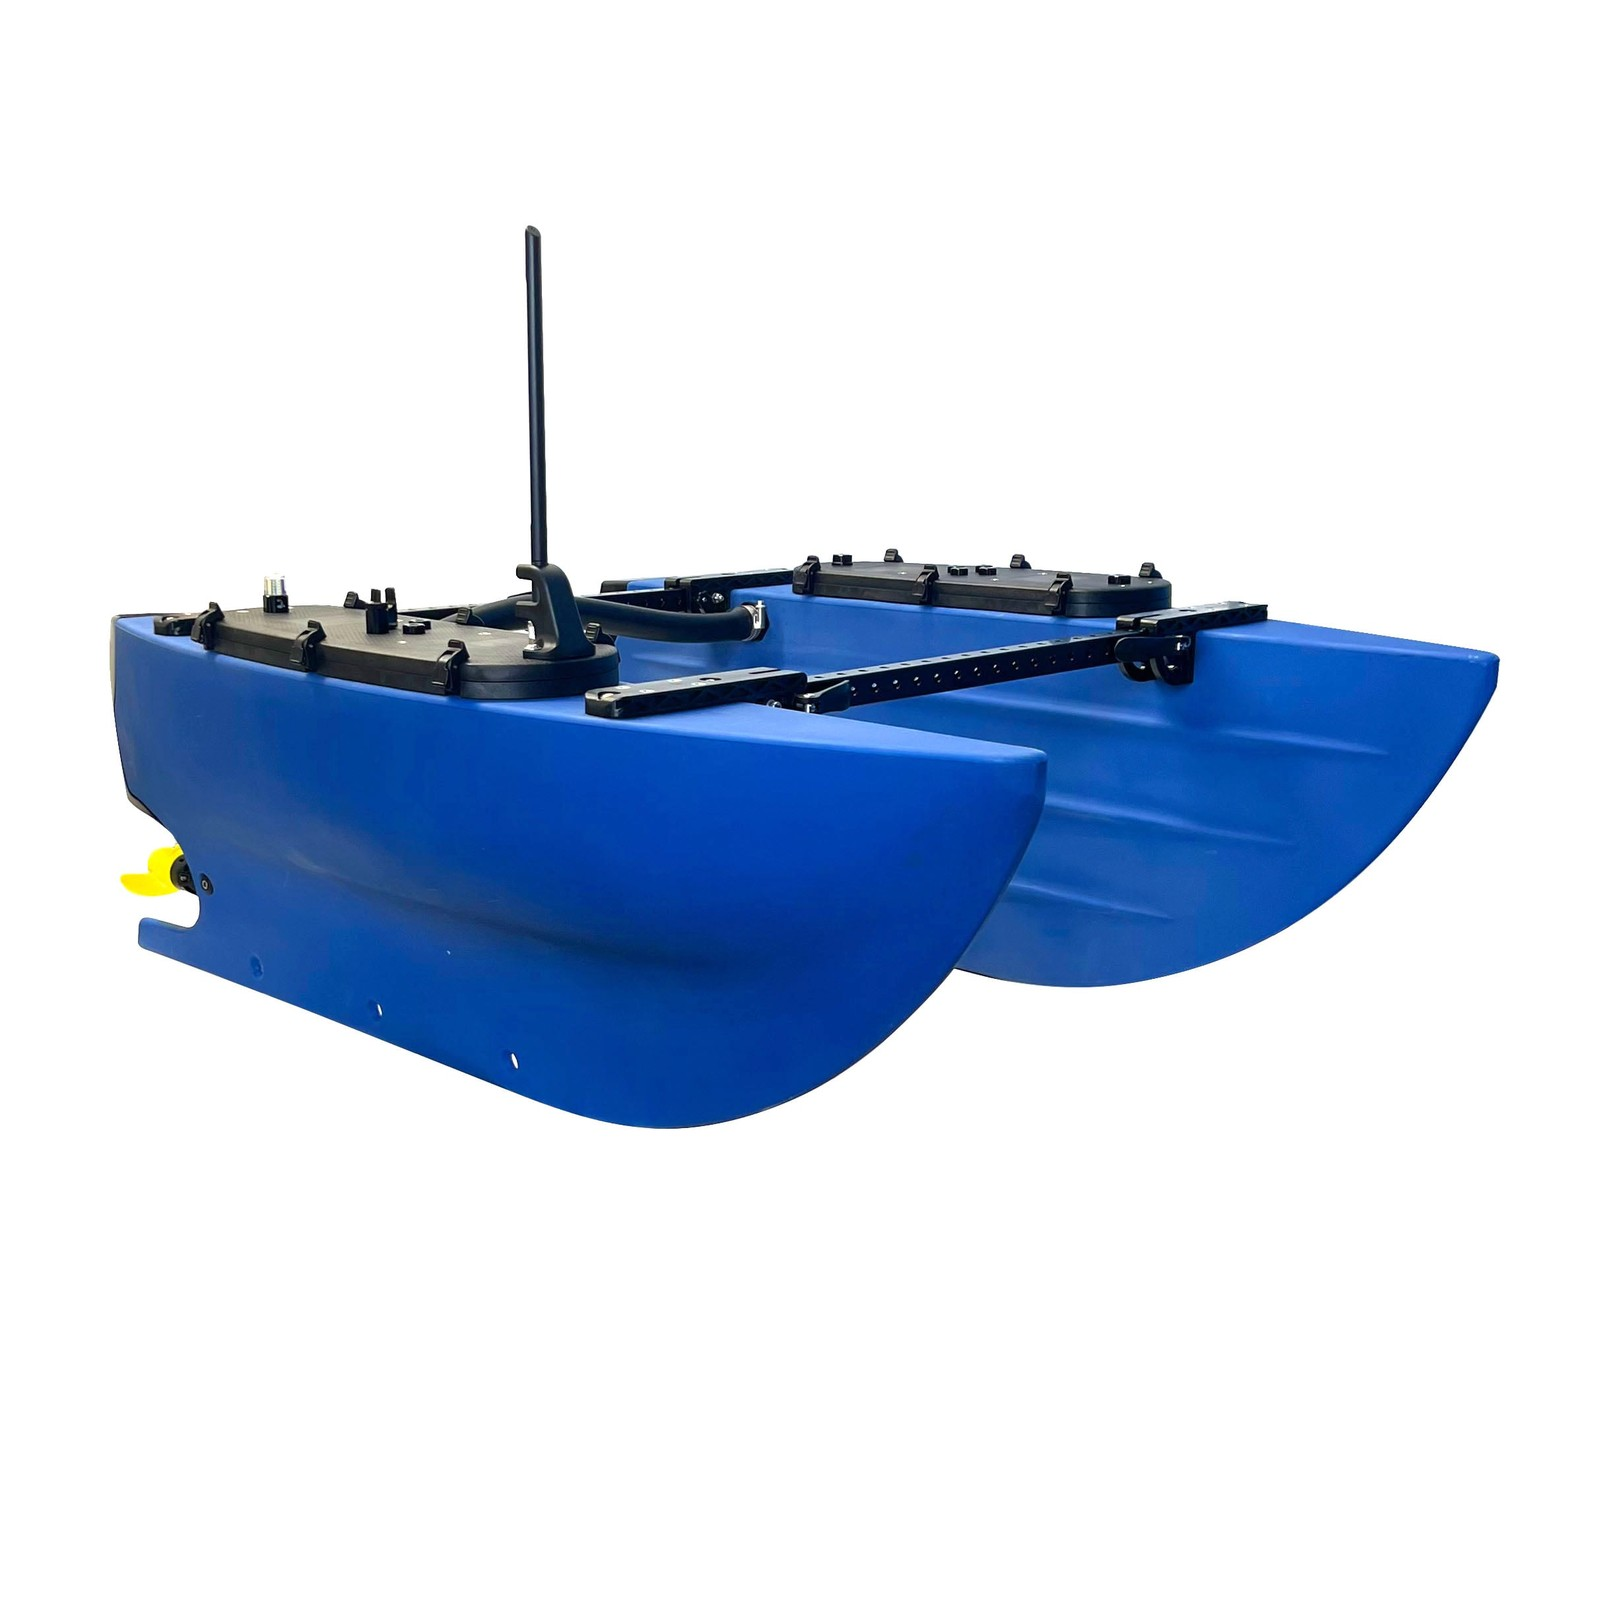
\includegraphics[height=2.0cm, keepaspectratio]{blueboat.jpg}\\
        \vspace{0.15em}
        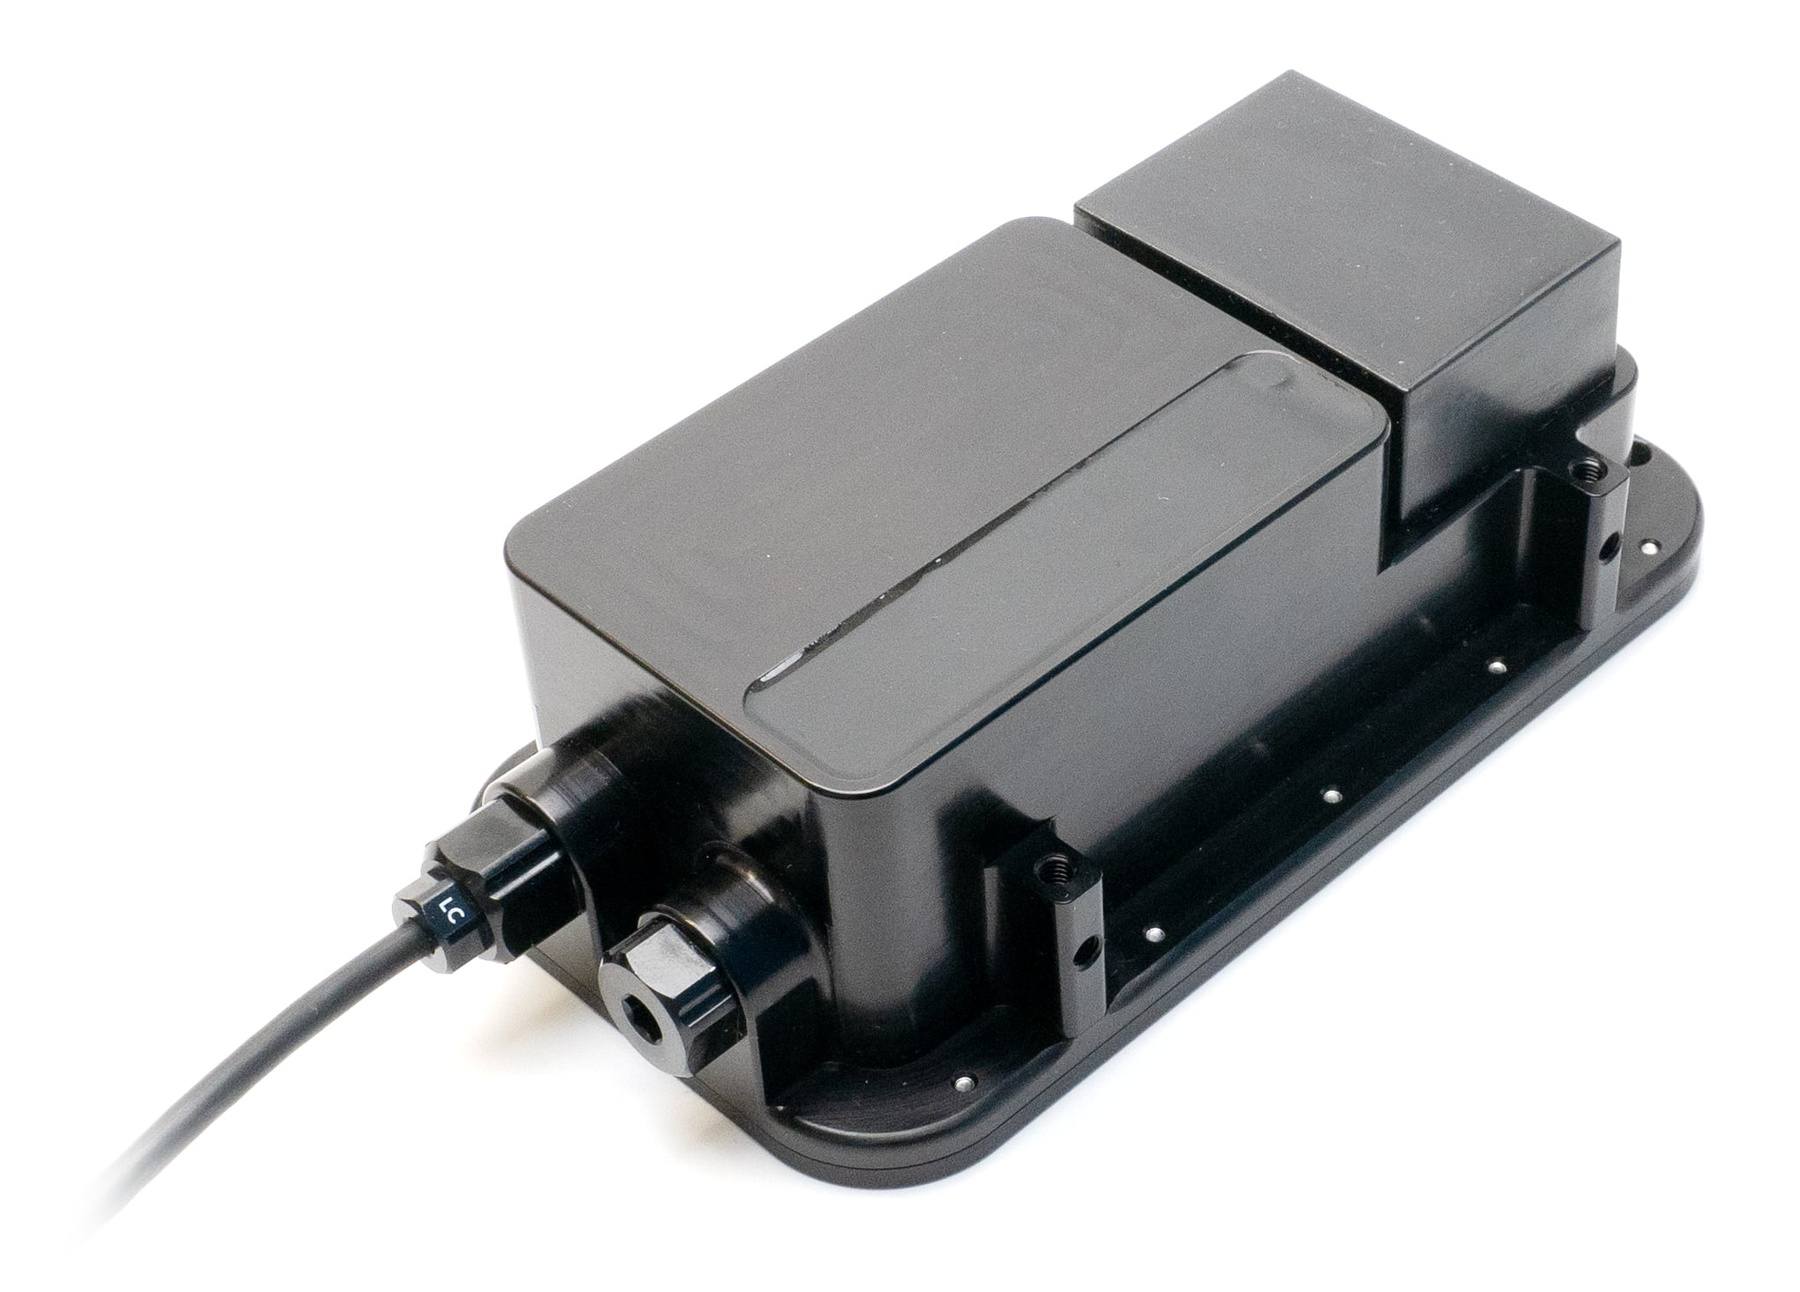
\includegraphics[height=1.7cm, keepaspectratio]{cerulean_surveyor_mbes.jpg}\\
        \vspace{0.1em}
        \scriptsize\textbf{BlueBoat} + \textbf{MBES Surveyor 240-16}
      \end{center}
    \end{column}

    \begin{column}{0.62\textwidth}
      \textbf{Cartographie bathymétrique \& physico-chimique} :
      \scriptsize
      \begin{itemize}
        \item Coque catamaran BlueBoat pilotée par \tech{ArduRover}.
        \item \textbf{Positionnement centimétrique} : GNSS RTK connecté au réseau public \succw{Centipede RTK}.
        \item \textbf{Sondeur sous coque} : Ping Sonar ou Cerulean Surveyor (MBES multifaisceaux) pour MNT 3D haute résolution.
        \item \textbf{Mission type} : tracé de transects parallèles espacés de $5\,\text{m}$, quadrillage automatique à $1.5\,\text{m/s}$ pendant 6 heures.
      \end{itemize}

      \vspace{0.3em}
      \begin{block}{Atouts Opérationnels}
        \scriptsize
        Déploiement par 1 seule personne sans grue, zéro risque d'immersion caisson, rapatriement WiFi/4G en direct au labo.
      \end{block}
    \end{column}
  \end{columns}
\end{frame}

\begin{frame}{5.3 Cas Pratique 3 : Équipe Mixte ASV-ROV (BlueBoat + BlueROV2)}
  \begin{columns}[T]
    \begin{column}{0.48\textwidth}
      \begin{center}
        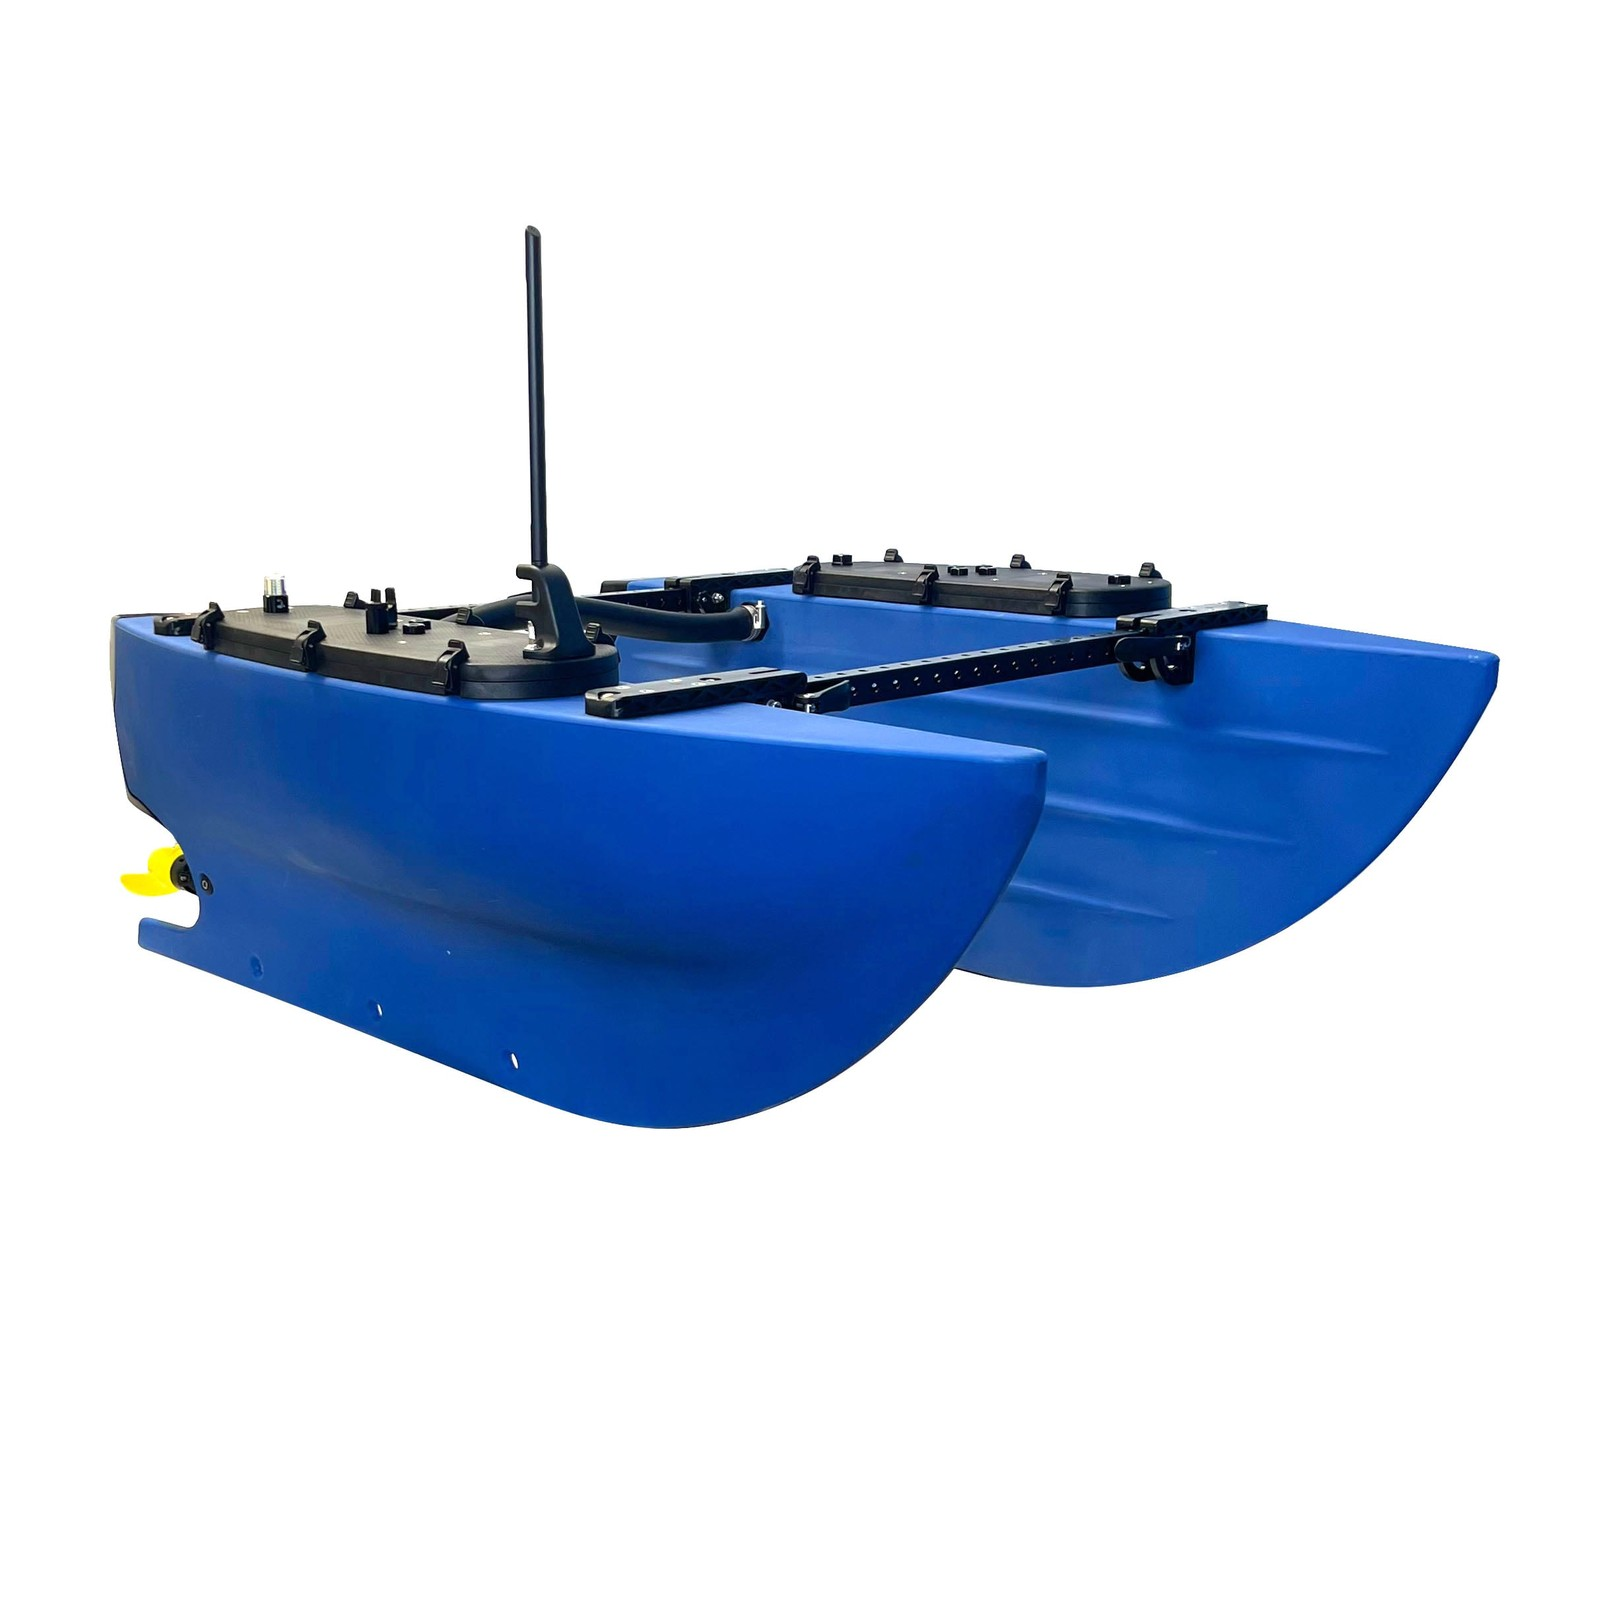
\includegraphics[height=1.5cm, keepaspectratio]{blueboat.jpg}
        \hspace{0.2cm}
        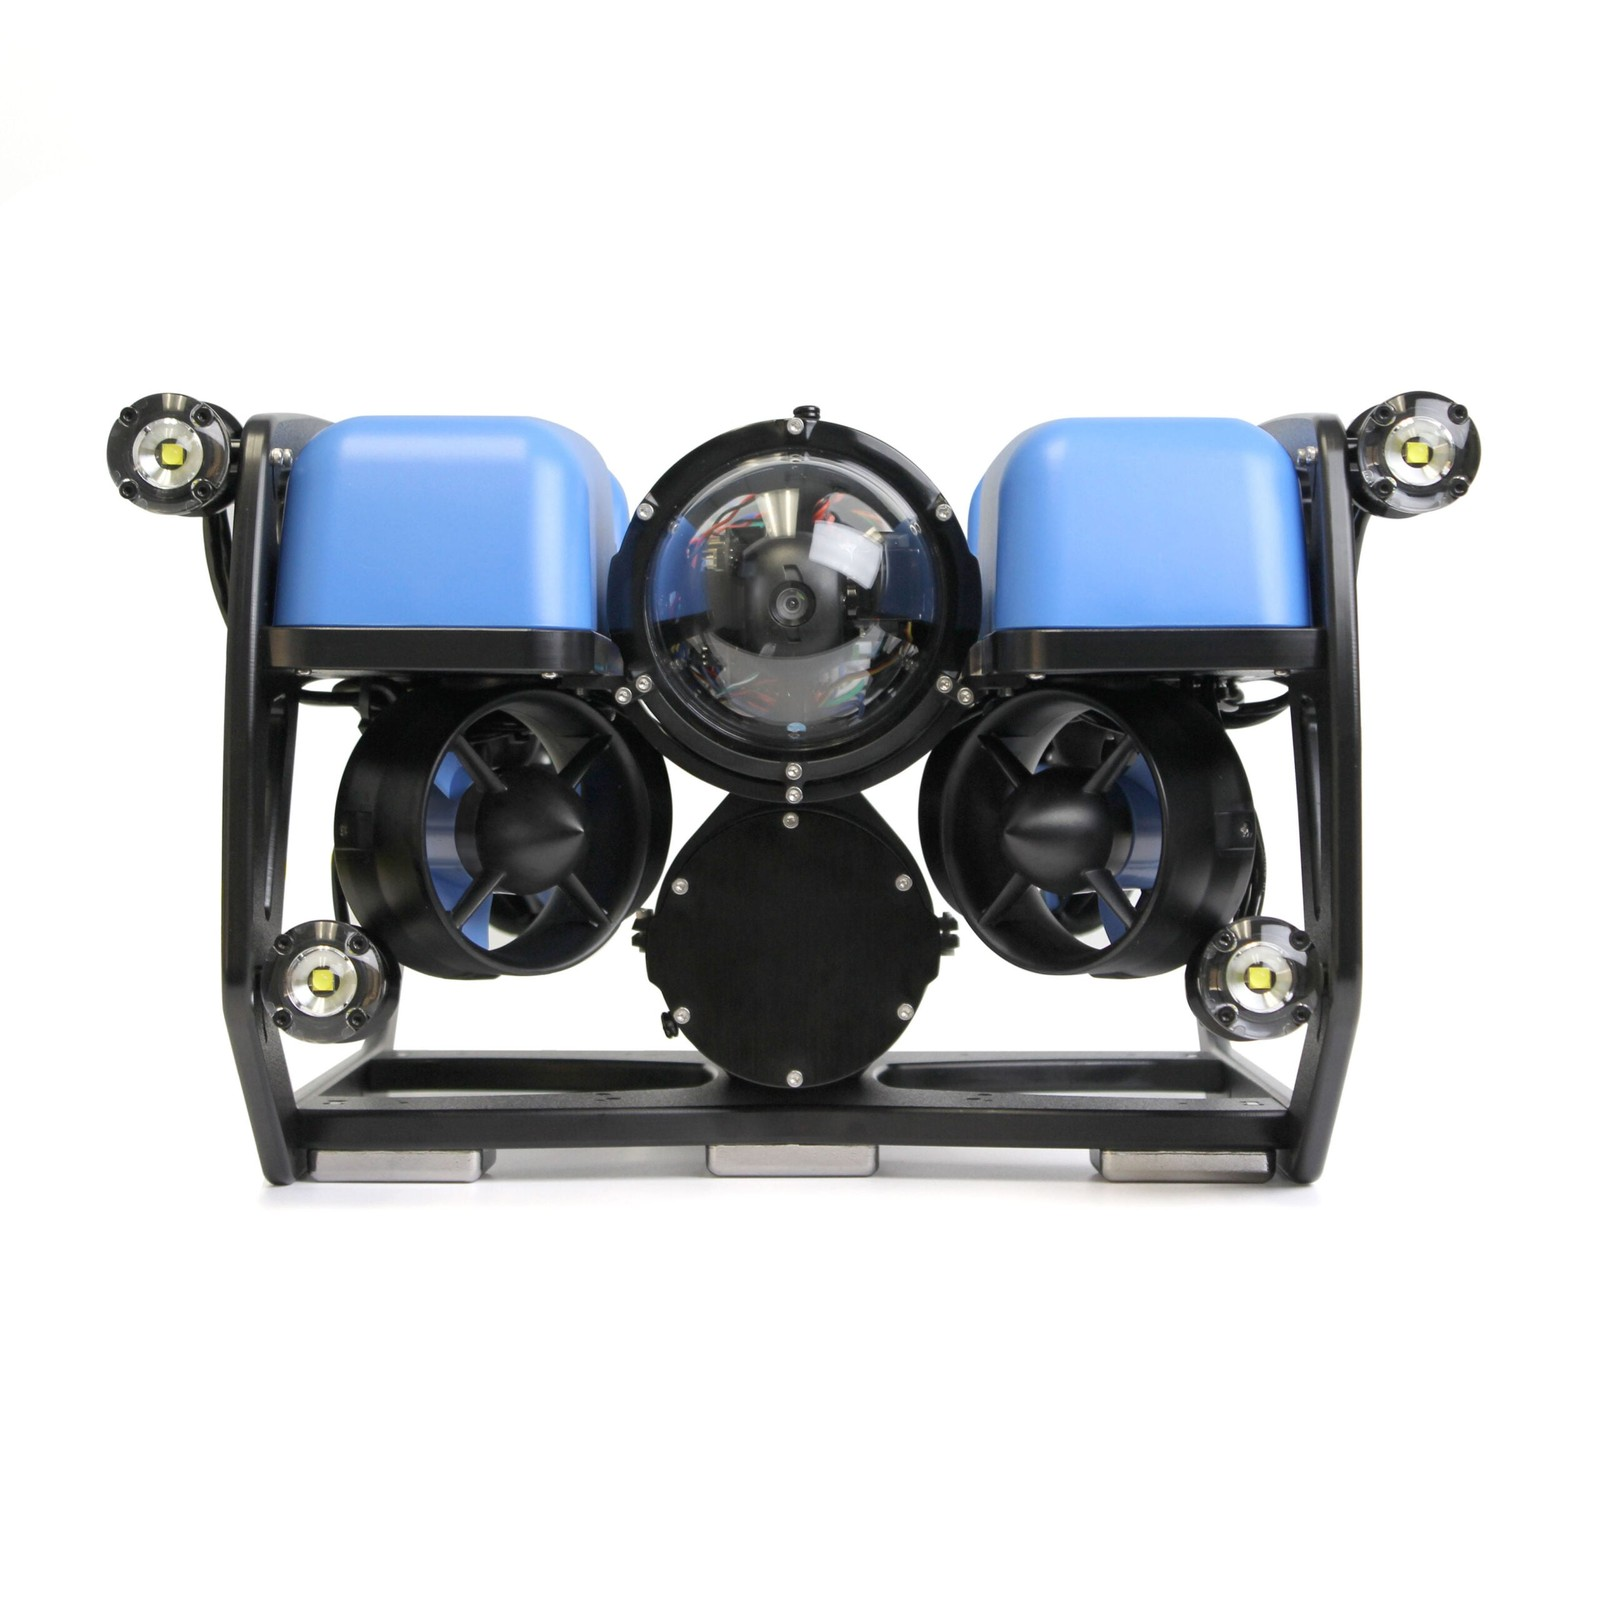
\includegraphics[height=1.5cm, keepaspectratio]{bluerov2.jpg}\\
        \vspace{0.1em}
        \tech{Drone de Surface ASV (BlueBoat)} + \succw{ROV Subaquatique (BlueROV2)}
      \end{center}
      \scriptsize
      \begin{block}{Le Cœur du Concept : La Passerelle de Surface}
        \begin{itemize}
          \item Le \textbf{BlueBoat} (ASV) navigue de façon autonome sur la zone d'étude grâce au positionnement \textbf{GNSS}.
          \item Il transporte éventuellement un enrouleur d'ombilical, l'antenne Wi-Fi/4G et un modem acoustique USBL.
        \end{itemize}
      \end{block}
    \end{column}

    \begin{column}{0.50\textwidth}
      \begin{exampleblock}{Avantages de l'Équipe Mixte Air-Surface-Fond}
        \scriptsize
        \begin{itemize}
          \item \textbf{Déploiement à grande élongation} : l'ASV amène le ROV sur site sans mobiliser de navire de recherche lourd avec équipage.
          \item \textbf{Relais de données haut débit} : le BlueBoat sert de répéteur radio/4G vers le laboratoire à terre.
          \item \textbf{Recalage absolu} : l'ASV injecte sa position GNSS RTK par USBL dans l'estime du BlueROV2.
        \end{itemize}
      \end{exampleblock}
    \end{column}
  \end{columns}
\end{frame}

\begin{frame}{5.4 Cas Pratiques Innovants : MAUV \& Flagellator}
  \begin{columns}[T]
    \begin{column}{0.47\textwidth}
      \begin{center}
        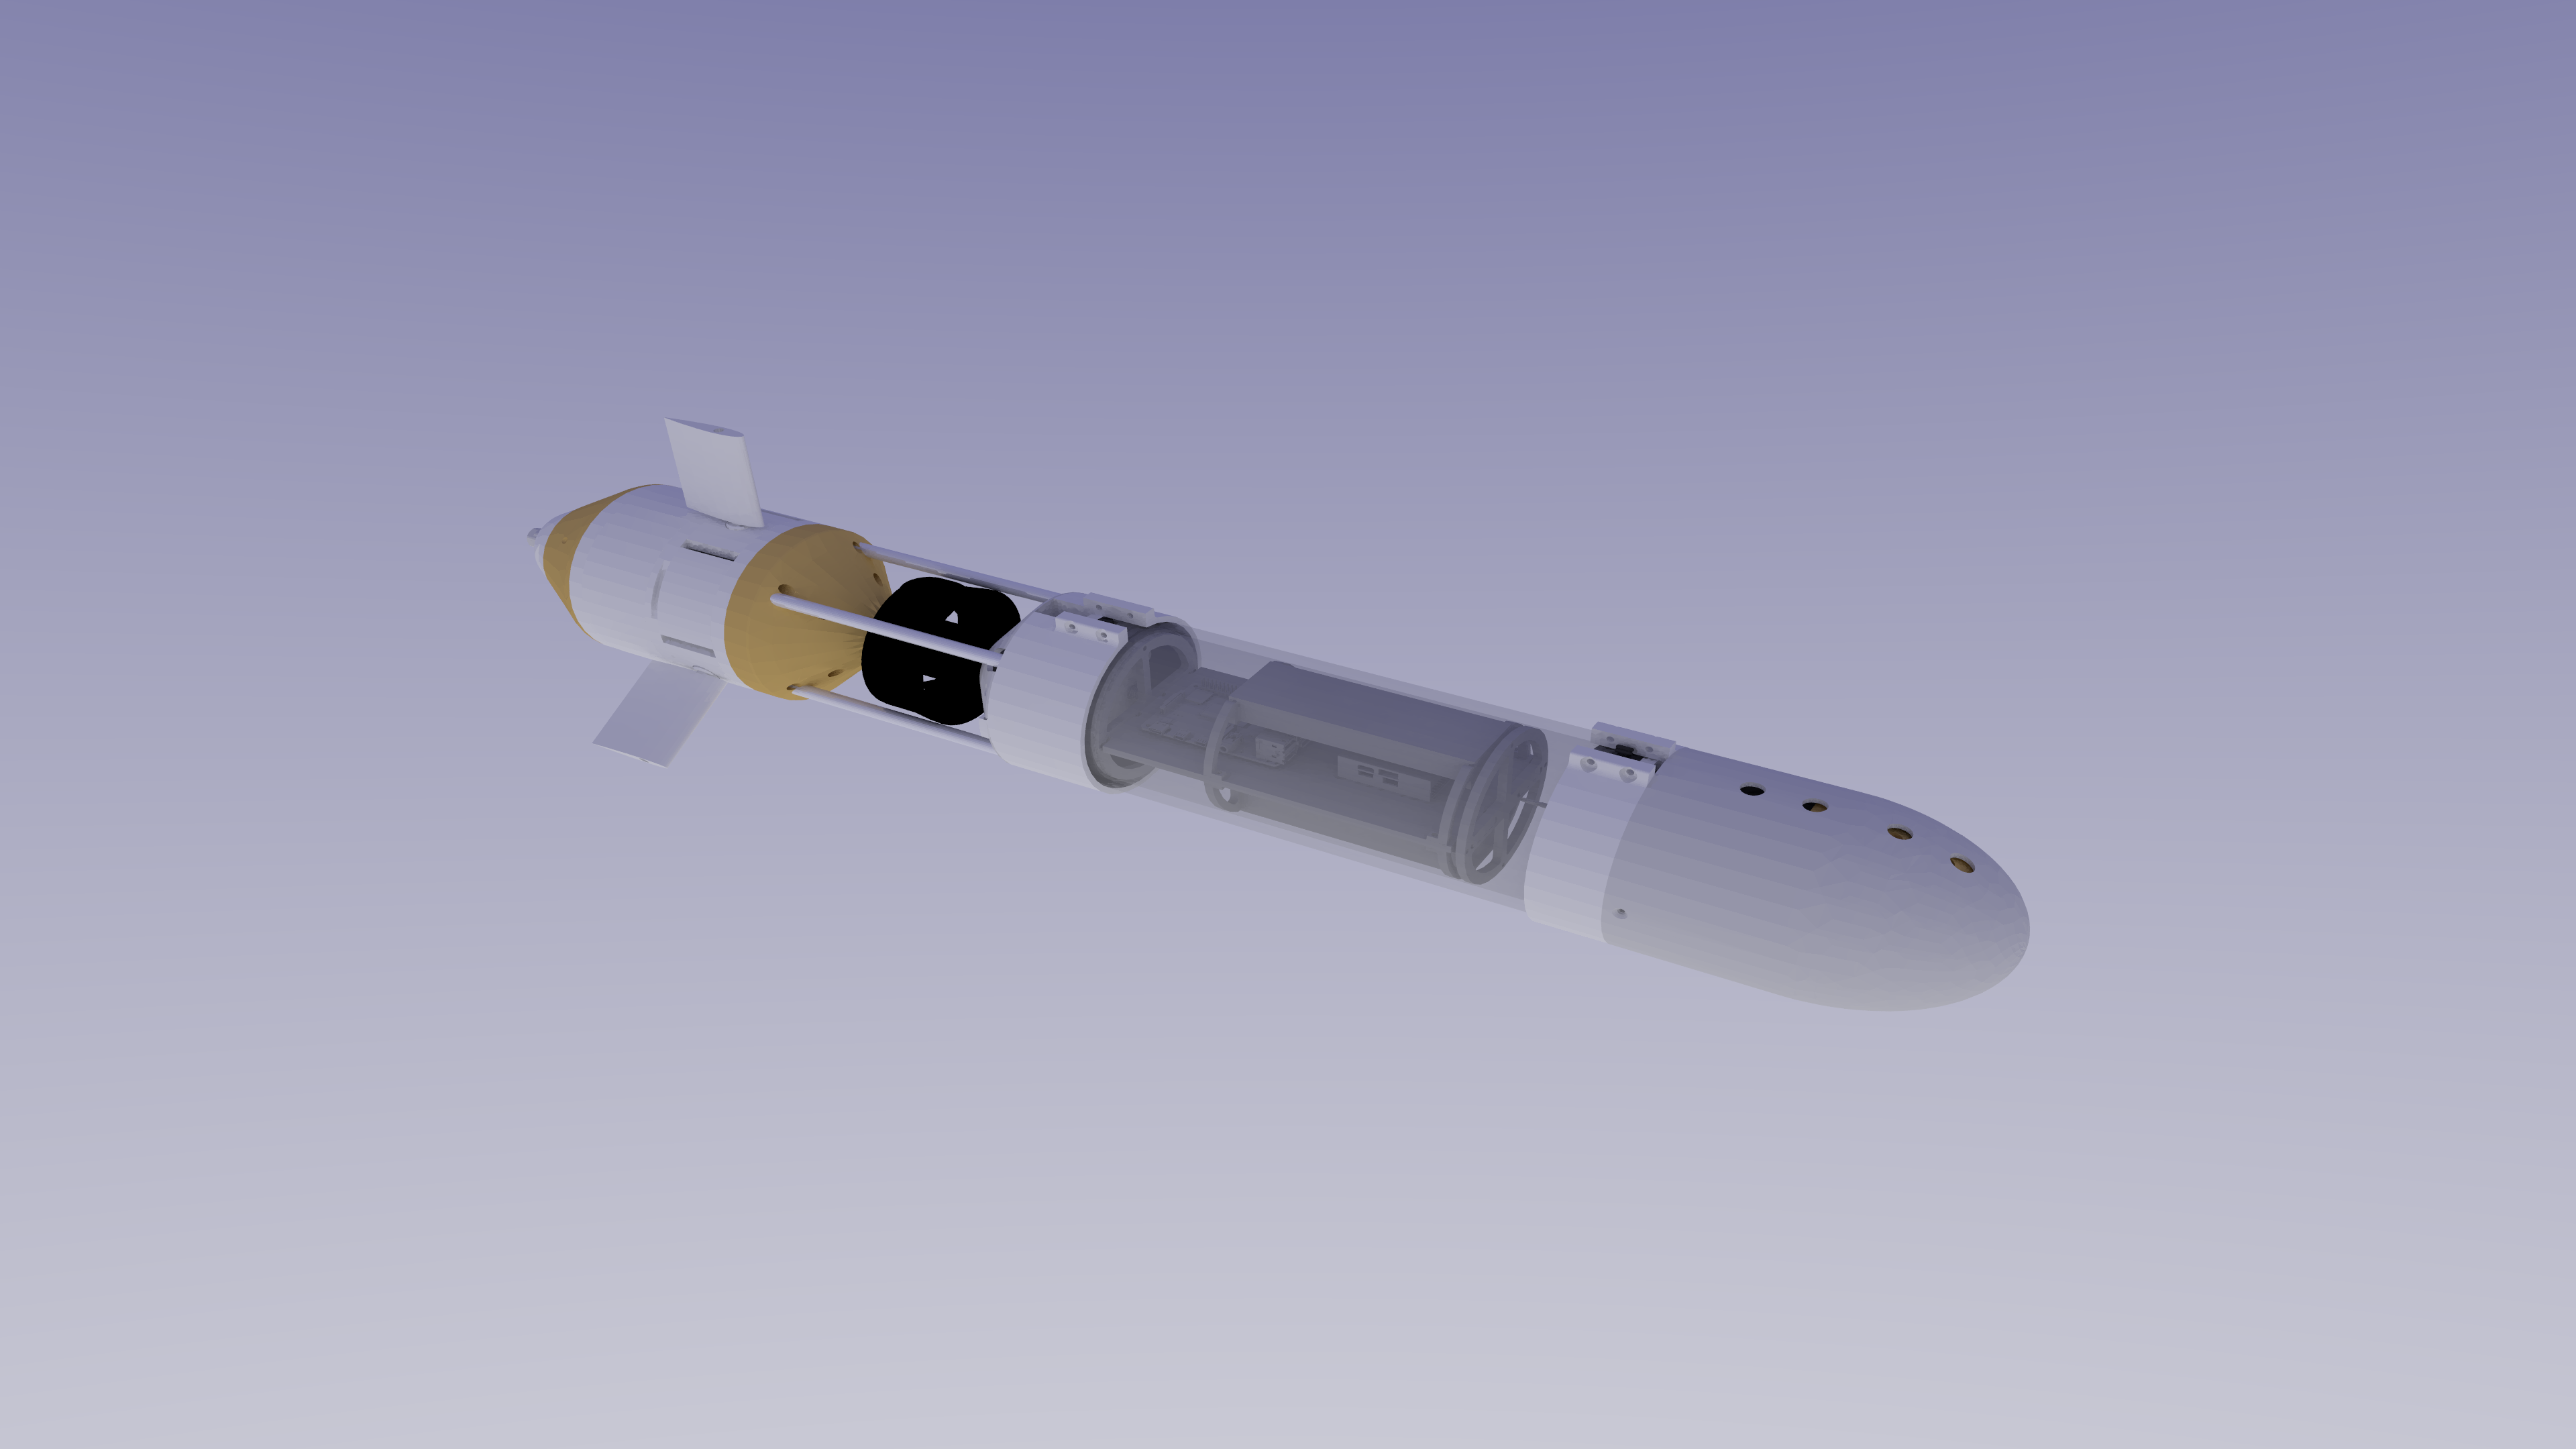
\includegraphics[height=2.1cm, keepaspectratio]{mauv.png}\\
        \vspace{0.1em}
        \tech{Modular-AUV (MAUV)}\\
        \tiny\textit{Vecteur sous-marin modulaire ultra-léger}
      \end{center}
      \scriptsize
      \begin{itemize}
        \item \textbf{Concept MAUV} : sous-marins ultra-léger ($<15\,\text{kg}$).
        \item \textbf{Man\oe uvrant} : propulseur placé devant les ailerons pour générer un flux d'eau permettant de tourner à vitesse très faible.
      \end{itemize}
    \end{column}

    \begin{column}{0.47\textwidth}
      \begin{center}
        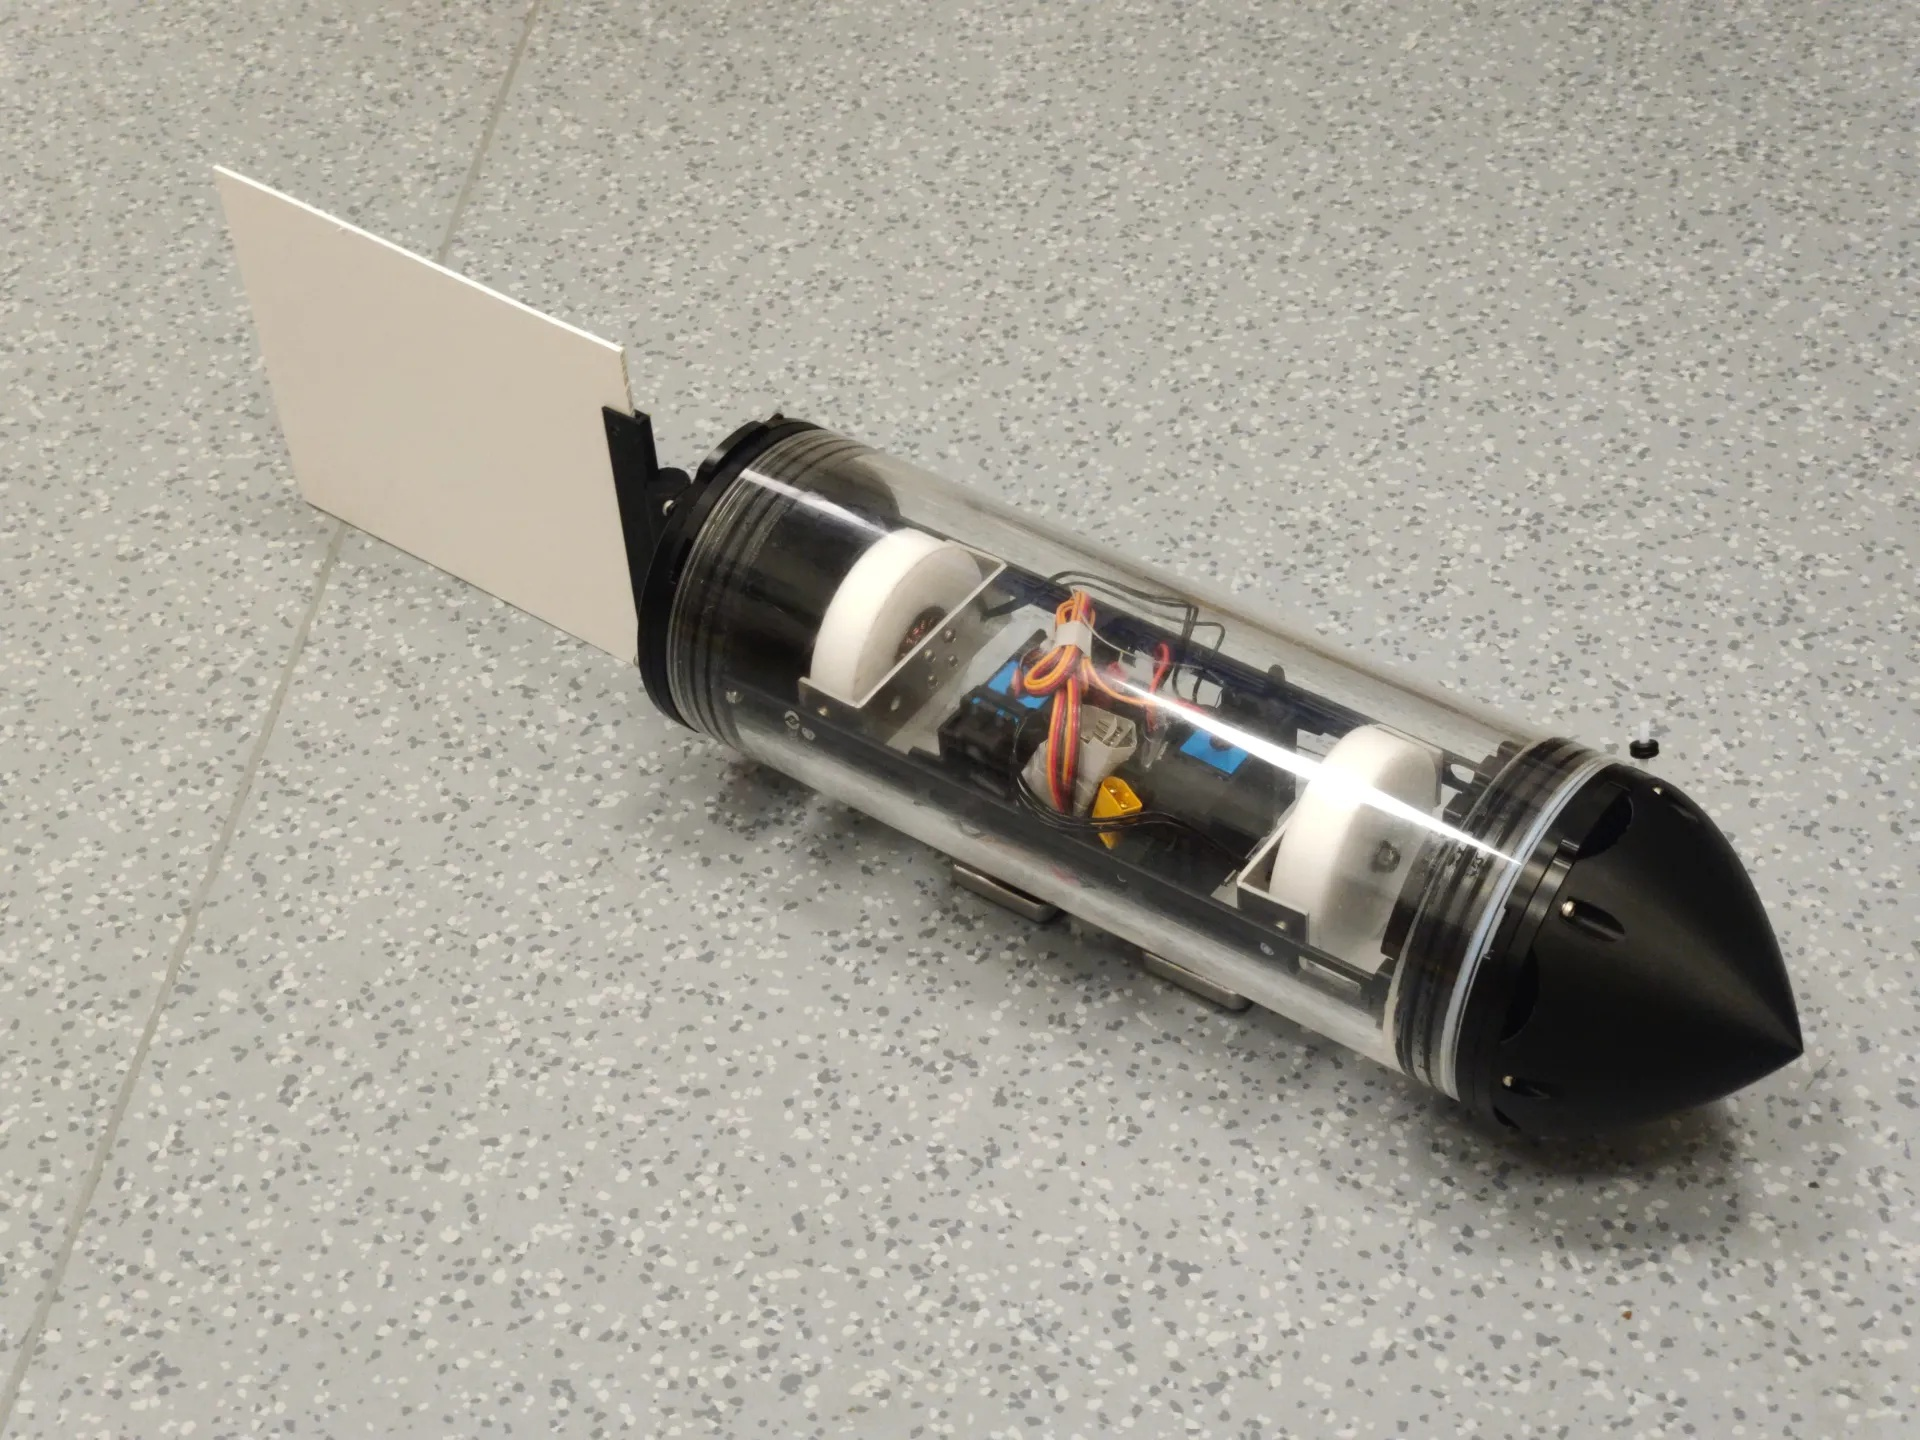
\includegraphics[height=2.1cm, keepaspectratio]{flagellator.jpg}\\
        \vspace{0.1em}
        \alertw{Le Robot Bio-inspiré Flagellator}\\
        \tiny\textit{Propulsion ondulatoire flagellaire}
      \end{center}
      \scriptsize
      \begin{itemize}
        \item \textbf{Nage biomimétique} : propulsion par ondulation continue d'une membrane/flagelle déformable.
        \item \textbf{Zéro hélice contondante} : intégrité et sécurité absolue lors des interventions près de la faune ou des récifs fragiles.
        \item \textbf{Pas d'étanchéité} : absence de passage de cable pour les actionneurs.
      \end{itemize}
    \end{column}
  \end{columns}
\end{frame}

\begin{frame}{5.4 Atelier Collaboratif : À Vous la Parole !}
  \begin{block}{Tour de table des projets scientifiques Drone\&Cap' \& 2RM}
    Présentez en 2 minutes votre problématique d'instrumentation :
    \begin{itemize}
      \item Quel est votre \textbf{milieu d'étude} ? (lagune côtière, récif corallien, fleuve turbide, lac de haute montagne).
      \item Quelles sont les \textbf{grandeurs physiques} à mesurer ? (bathymétrie, herbiers, turbidité, traceurs chimiques, profils CTD).
      \item Quel est le compromis optimal : \textbf{ROV filaire}, \textbf{AUV autonome} ou \textbf{ASV de surface} ?
    \end{itemize}
  \end{block}

  \vspace{0.6em}
  \begin{exampleblock}{Questions \& Réponses Ouvertes}
    \begin{itemize}
      \item Conseils sur l'approvisionnement et l'intégration mécanique/logicielle.
      \item Retours d'expérience sur les pièges à éviter lors des premières campagnes en mer.
      \item Partage de briques logicielles au sein des réseaux Drone\&Cap' et 2RM.
    \end{itemize}
  \end{exampleblock}

\end{frame}
